Google Chromecast es un dispositivo de reproducción multimedia fabricado por Google. Reproduce audio/video conectado con una televisión o monitor por HDMI haciendo streaming mediante Wi-Fi. Un nuevo modelo que soporta resolución 4k será lanzado en Noviembre de 2016.

Para enviar la información utiliza Google Cast, seleccionamos el contenido que queremos reproducir por una aplicación (Android 4.1+, iOS 7.0+) o mediante el navegador chrome y se carga por su puerto mico-USB.

\begin{figure}[h]
	\centering
	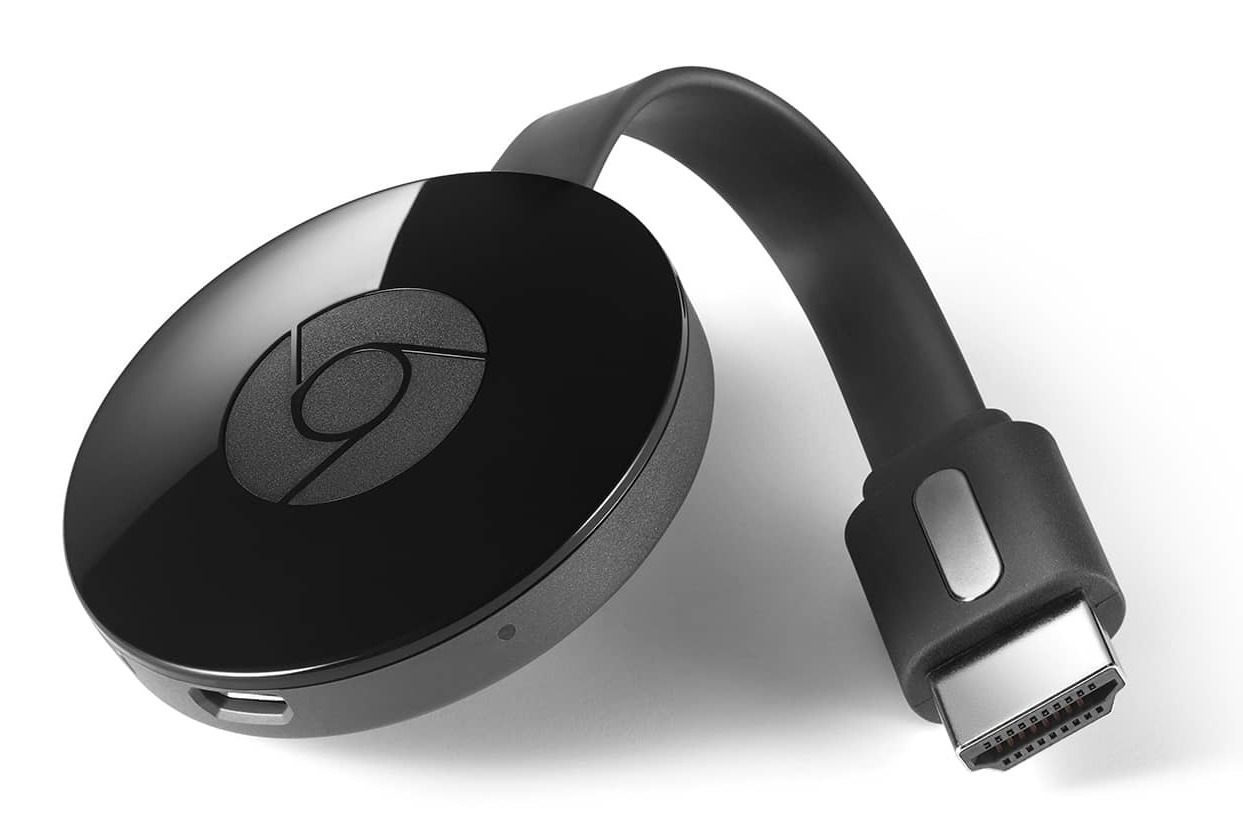
\includegraphics[width=0.5\textwidth]{./Memoria/Imagenes/Chromecast.jpg}
	\label{fig:chromecast}
\end{figure}

Para iniciar la reproducción pulsamos el botón de \textit{cast}, si el puerto HDMI dispone de Consumer Electronics Control (CEC) la televisión se encenderá inmediatamente.

El contenido reproducido puede ser accedido mediante Wi-fi o residir en el almacenamiento local del dispositivo.
Las imágenes o vídeos enviados mediante dispositivos Android suelen perder calidad, ya que las imágenes en pantallas pequeñas suelen ser escaladas.

Cuando no hay contenido en streaming reproduce un contenido personalizable de fondo, puede incluir fotos personales, de satélite, noticias, etc.

\begin{figure}[h]
	\centering
	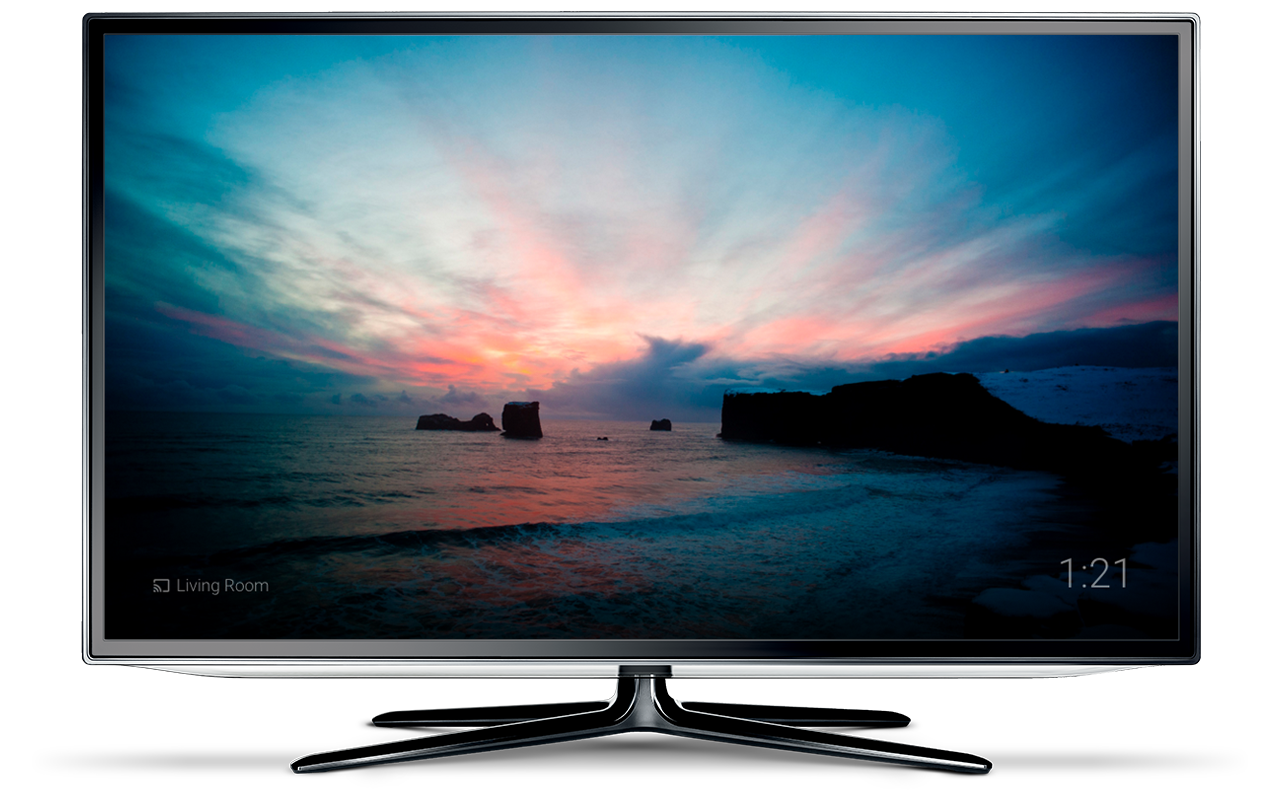
\includegraphics[width=0.7\textwidth]{./Memoria/Imagenes/fondo.png}
	\label{fig:fondo}
\end{figure}

